\documentclass[letterpaper]{article} % DO NOT CHANGE THIS
\usepackage{aaai2027}  % DO NOT CHANGE THIS
\usepackage[hyphens]{url}  % DO NOT CHANGE THIS
\usepackage{graphicx} % DO NOT CHANGE THIS
\urlstyle{rm} % DO NOT CHANGE THIS
\def\UrlFont{\rm}  % DO NOT CHANGE THIS
\usepackage{natbib}  % DO NOT CHANGE THIS AND DO NOT ADD ANY OPTIONS TO IT
\usepackage{caption} % DO NOT CHANGE THIS AND DO NOT ADD ANY OPTIONS TO IT
\frenchspacing  % DO NOT CHANGE THIS
\setlength{\pdfpagewidth}{8.5in} % DO NOT CHANGE THIS
\setlength{\pdfpageheight}{11in} % DO NOT CHANGE THIS
\usepackage{booktabs}
\usepackage{amsmath}
\pdfinfo{
/TemplateVersion (2027.2)
}
\nocopyright % course report, not an AAAI publication

\setcounter{secnumdepth}{0}


\title{ECE-GY 7123 Project 1 Report}
\author{
    Samarth Pusegaonkar
}
\affiliations{
    New York University\\
    ssp6681@nyu.edu
}

\begin{document}

\maketitle

\begin{abstract}
We design and train a residual network for CIFAR-10 image classification under a hard limit of 5 million trainable parameters, trained from scratch on the 50{,}000 provided images. Rather than hand-picking a model, we run a staged sweep over three axes, architecture, optimizer, and regularization, using short 15-epoch runs. We then retrain the strongest configurations for 150 epochs. The final model is a three-stage ResNet with 4.62M parameters that concentrates computation at high spatial resolution. Trained with SGD, a one-cycle learning-rate schedule, TrivialAugment, and random erasing, it reaches 97.06\% accuracy on a held-out validation split. Retrained on all 50{,}000 images, it scores 88.4\% on the public leaderboard.
\end{abstract}

\section{Introduction}

\subsection{The Competition}
The Efficient ResNet Architecture Challenge asks participants to build the most accurate CIFAR-10 classifier possible with a modified residual network of at most 5 million trainable parameters. CIFAR-10~\citep{krizhevsky2009cifar} consists of $32\times32$ RGB images from ten classes (airplane, automobile, bird, cat, deer, dog, frog, horse, ship, truck). The competition supplies 50{,}000 labeled training images and 2{,}000 unlabeled test images. All models must be trained from scratch: pretrained weights and external data are prohibited. Predictions are scored by classification accuracy on a hidden labeled test set, split equally into a public leaderboard, shown during the competition, and a private leaderboard that determines final rankings. The challenge is therefore not to build the largest network, but to decide where a fixed parameter budget is best spent and how to train it.

\subsection{Residual Networks}
ResNets~\citep{he2016resnet} make very deep convolutional networks trainable by wrapping groups of layers in a skip connection:
\begin{equation}
  y = \mathrm{ReLU}\big(F(x) + S(x)\big),
\end{equation}
where $F$ is a learned residual transformation and $S$ is the skip path. The skip path gives gradients a direct route to earlier layers, so adding blocks does not make optimization harder. In the \emph{BasicBlock} used here, $F$ is two $k\times k$ convolutions, each followed by batch normalization~\citep{ioffe2015bn}, with a ReLU between them. $S$ is the identity when input and output shapes match, and a $1\times1$ strided convolution with batch normalization (a projection) when the block changes resolution or width. Blocks are grouped into \emph{stages}; the first block of each later stage halves the spatial resolution and usually increases the channel count. A network is then defined by the number of stages, the width of each stage, the number of blocks per stage, and the kernel size $k$. These are the architectural knobs we tune.

\subsection{Training Techniques}
\paragraph{Optimizers.}
SGD with Nesterov momentum updates the weights along a running average of past gradients, evaluated at a look-ahead point. Adam~\citep{kingma2015adam} adapts a per-parameter step size from running estimates of the gradient's first and second moments. AdamW~\citep{loshchilov2019adamw} decouples weight decay from that adaptive step, which restores its regularizing effect. RMSProp~\citep{tieleman2012rmsprop} divides each gradient by a running average of its recent magnitude.

\paragraph{One-cycle learning-rate schedule.}
The one-cycle policy~\citep{smith2019superconvergence} raises the learning rate from a small value to a peak $\eta_{\max}$ over the first part of training, then anneals it to nearly zero by the final step, cycling momentum in the opposite direction. The high-learning-rate phase acts as a regularizer, and the final annealing phase settles the model into a good minimum. Because the schedule is defined by the total number of steps, a run of any length ends fully annealed.

\paragraph{TrivialAugment.}
TrivialAugment~\citep{muller2021trivialaugment} applies a single image operation to each training sample. The operation is drawn uniformly from a fixed set, such as rotation, shear, translation, color, contrast, brightness, sharpness, posterize, solarize, and equalize, and applied at a uniformly random strength. Unlike earlier automatic augmentation methods, it requires no search or tuning, yet matches or beats them on CIFAR-10.

\paragraph{Random erasing.}
Random erasing~\citep{zhong2020randomerasing} replaces a randomly sized and placed rectangle of each training image, with probability $p$, by random values. This forces the network to rely on more than one discriminative region and simulates occlusion.

\paragraph{Label smoothing.}
Label smoothing~\citep{szegedy2016inception} trains against a target that mixes the one-hot label with the uniform distribution: $(1-\epsilon)$ on the true class and $\epsilon/10$ spread over all classes. This discourages over-confident logits. With $\epsilon=0.1$, the cross-entropy cannot fall below about $0.5$, a fact we use to diagnose memorization.

\paragraph{Weight decay and dropout.}
Weight decay penalizes large weights. Dropout~\citep{srivastava2014dropout} randomly zeroes activations during training. We apply it only before the final classifier, since batch normalization already regularizes the convolutional layers.

\paragraph{Test-time augmentation.}
At inference, we average the network's logits over an image and its horizontal mirror.

\section{Methodology}

\paragraph{Data and validation.}
We hold out a fixed random 5{,}000 of the 50{,}000 training images (seed 0) for validation and train on the remaining 45{,}000. Inputs are normalized with the CIFAR-10 per-channel mean and standard deviation. At evaluation we apply horizontal-flip test-time augmentation (TTA), summing the logits of each image and its mirror. With 5{,}000 validation images, the standard error of an accuracy near 92\% is about 0.4 points, so we treat smaller differences between single runs as ties.

\paragraph{Default training recipe.}
Unless a sweep changes it, every run uses batch size 256, SGD with Nesterov momentum 0.9, peak learning rate 0.1, weight decay $5\times10^{-4}$, and cross-entropy with label smoothing 0.1. The one-cycle schedule uses PyTorch defaults: 30\% warm-up from $\eta_{\max}/25$, cosine annealing to $\eta_{\max}/10^{4}$, and momentum cycled between 0.85 and 0.95. Augmentation is a random crop from a 4-pixel reflect-padded image, a horizontal flip, TrivialAugment, and random erasing with $p=0.25$. Each run uses the same seed and split, so differences between runs reflect only the configuration. Training ran in fp32 on an Apple-silicon GPU (PyTorch MPS backend).

\paragraph{Sweep procedure.}
A full grid over every factor was infeasible on our hardware: one 15-epoch run takes 7--28 minutes. We therefore ran a greedy coordinate search along three axes, in order. Each axis is swept with 15-epoch runs while all other settings stay at the incumbent best. Because the one-cycle schedule completes within each run, short runs are fully annealed rather than truncated. At each stage, the winner is chosen over the union of the current and all previous stages, so a change is adopted only if it beats the incumbent. After the sweep, the two best distinct configurations are retrained for 150 epochs. Every run is appended, with its configuration and per-epoch curves, to a results log. This makes the sweep resumable and every table in this report reproducible from a single notebook.

\paragraph{Axis 1: architecture.}
We compare six layouts of 4.3--4.9M parameters, each built from the same template: a $3\times3$ stem convolution, stages of BasicBlocks, global average pooling, optional dropout, and a linear classifier (Table~\ref{tab:archs}). Each layout tests a different way to spend the budget: more depth, more width, more computation early, an extra downsampling stage, or larger kernels.

\begin{table}[t]
\centering
\small
\setlength{\tabcolsep}{4pt}
\begin{tabular}{lllcr}
\toprule
Layout & Widths & Blocks & $k$ & Params \\
\midrule
base         & 64-128-256    & 3-4-3   & 3 & 4.62M \\
deep-narrow  & 48-96-192     & 6-6-5   & 3 & 4.39M \\
wide-shallow & 96-192-320    & 2-2-2   & 3 & 4.90M \\
early-heavy  & 96-160-256    & 4-4-2   & 3 & 4.62M \\
4-stage      & 48-96-192-288 & 1-2-2-2 & 3 & 4.32M \\
large-kernel & 40-80-160     & 2-3-3   & 5 & 4.58M \\
\bottomrule
\end{tabular}
\caption{Architecture candidates. Widths are channels per stage, starting at $32\times32$ resolution and halving per stage.}
\label{tab:archs}
\end{table}

\paragraph{Axis 2: optimizer.}
On the best architecture, we compare SGD with Nesterov momentum at peak learning rates $\{0.05, 0.1, 0.2\}$, AdamW at $\{10^{-3}, 3\times10^{-3}\}$ with decoupled weight decay $5\times10^{-2}$, and RMSProp (momentum 0.9) at $\{3\times10^{-4}, 10^{-3}\}$. Each optimizer gets its own learning-rate range, since a single shared value would unfairly favor one of them.

\paragraph{Axis 3: regularization.}
On the best architecture and optimizer, we vary weight decay ($\times0.3$ and $\times3$ the incumbent), add dropout 0.2 before the classifier, and weaken augmentation, either to crop + flip only or to crop + flip + TrivialAugment without random erasing. Label smoothing was held fixed at 0.1 throughout.

\section{Results}

\paragraph{Sweep outcomes.}
Table~\ref{tab:sweep} lists every sweep run.

\emph{Architecture:} at matched parameter counts, accuracy tracks computation at high resolution. The early-heavy layout, which keeps four wide blocks at both $32\times32$ and $16\times16$, wins. The 4-stage model, which places most of its parameters at $4\times4$, is fastest but worst. A deeper, thinner network and larger kernels, which spend parameters on spatial extent rather than channels, both lose.

\emph{Optimizer:} SGD with Nesterov momentum is best and improves with a higher peak learning rate. AdamW comes within 0.5 points. RMSProp is unstable under the one-cycle schedule and collapses at the higher rate.

\emph{Regularization:} weight decay and dropout changes are within noise. Weaker augmentation looks clearly better at 15 epochs.

\begin{table}[t]
\centering
\small
\setlength{\tabcolsep}{4pt}
\begin{tabular}{llrr}
\toprule
Axis & Setting & Val (\%) & Min \\
\midrule
Arch. & early-heavy           & \textbf{92.10} & 24.1 \\
      & wide-shallow          & 91.82 & 16.3 \\
      & base                  & 91.40 & 14.0 \\
      & deep-narrow           & 90.70 & 17.0 \\
      & large-kernel          & 90.44 & 18.8 \\
      & 4-stage               & 90.10 & 7.4 \\
\midrule
Opt.  & SGD, $\eta$=0.2       & \textbf{92.40} & 28.1 \\
      & SGD, $\eta$=0.1       & 92.10 & 24.1 \\
      & SGD, $\eta$=0.05      & 91.68 & 24.1 \\
      & AdamW, $\eta$=3e-3    & 91.92 & 26.6 \\
      & AdamW, $\eta$=1e-3    & 91.38 & 25.9 \\
      & RMSProp, $\eta$=3e-4  & 88.78 & 21.7 \\
      & RMSProp, $\eta$=1e-3  & 80.20 & 21.0 \\
\midrule
Reg.  & crop + flip only      & \textbf{93.82} & 20.9 \\
      & + TrivialAug.\ (no erasing) & 92.64 & 21.3 \\
      & incumbent (full aug.) & 92.40 & 28.1 \\
      & weight decay $\times3$ & 92.28 & 21.1 \\
      & dropout 0.2           & 92.08 & 21.3 \\
      & weight decay $\times0.3$ & 91.82 & 21.3 \\
\bottomrule
\end{tabular}
\caption{All 15-epoch sweep runs (validation accuracy with flip TTA, and wall-clock minutes). Each axis starts from the previous axis's winner.}
\label{tab:sweep}
\end{table}

\paragraph{Long runs reverse the augmentation ranking.}
We retrained the two best distinct configurations (crop + flip only, and crop + flip + TrivialAugment) for 150 epochs (Table~\ref{tab:final}, Figure~\ref{fig:curves}). The ranking reverses: TrivialAugment reaches 96.96\% against 95.78\% for crop + flip. Without TrivialAugment, training loss falls to ${\approx}0.50$, close to the minimum achievable with label smoothing 0.1, meaning the network has essentially memorized its training set. With TrivialAugment it stays at 0.66. In short runs, strong augmentation mainly slows fitting; its regularizing benefit appears only once the model has enough epochs to overfit without it. Short proxy runs are therefore useful for choosing architecture and optimizer, but augmentation strength must be chosen at the target training length. Because of this, we also trained the full augmentation (with random erasing) for 150 epochs as a follow-up run. It reached 97.06\%, slightly above TrivialAugment alone, with a final training loss of 0.70, so random erasing was kept.

\begin{figure*}[t]
\centering
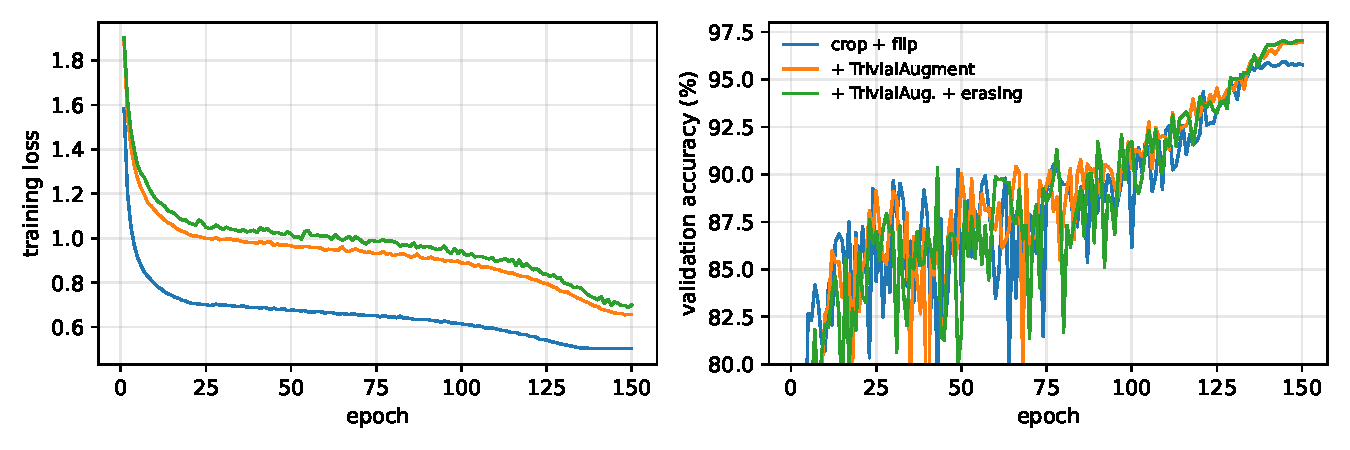
\includegraphics[width=0.85\textwidth]{curves.pdf}
\caption{Training loss and validation accuracy of the three 150-epoch runs. Most of the accuracy gain arrives as the one-cycle schedule anneals the learning rate in the final third of training.}
\label{fig:curves}
\end{figure*}

\paragraph{Final model and settled choices.}
The final model is the \textbf{early-heavy} ResNet (Table~\ref{tab:model}) with 4,621,354 trainable parameters, below the 5M limit. The settled choices are:
\begin{itemize}
  \item \textbf{Architecture:} widths 96-160-256, blocks 4-4-2, $3\times3$ kernels, identity skips with $1\times1$ projections at stage transitions, and no dropout.
  \item \textbf{Optimizer:} SGD with Nesterov momentum 0.9, one-cycle schedule with peak learning rate 0.2, and batch size 256.
  \item \textbf{Regularization:} weight decay $5\times10^{-4}$ and label smoothing 0.1.
  \item \textbf{Augmentation:} random crop, horizontal flip, and TrivialAugment, and random erasing with $p=0.25$.
  \item \textbf{Inference:} horizontal-flip TTA.
\end{itemize}
For submission, the best configuration is retrained on all 50{,}000 images, with no validation holdout, for 250 epochs. Table~\ref{tab:final} reports validation and public-leaderboard accuracy for each long run. The TrivialAugment model (96.96\% validation) scored 88.2\% on the public leaderboard; the final model scored 88.4\%.

\begin{table}[t]
\centering
\small
\setlength{\tabcolsep}{3pt}
\begin{tabular}{lccr}
\toprule
Stage & Output & Blocks & Params \\
\midrule
Stem    & $96{\times}32{\times}32$  & $3{\times}3$ conv & 2,784 \\
Stage 1 & $96{\times}32{\times}32$  & 4 & 665,088 \\
Stage 2 & $160{\times}16{\times}16$ & 4 & 1,769,280 \\
Stage 3 & $256{\times}8{\times}8$   & 2 & 2,181,632 \\
Head    & 10 & pool + linear & 2,570 \\
\midrule
Total   & & & \textbf{4,621,354} \\
\bottomrule
\end{tabular}
\caption{Final early-heavy architecture.}
\label{tab:model}
\end{table}

\begin{table}[t]
\centering
\small
\setlength{\tabcolsep}{3pt}
\begin{tabular}{lrrr}
\toprule
Run (150 ep.\ unless noted) & Val (\%) & Loss & LB (\%) \\
\midrule
crop + flip                 & 95.78 & 0.502 & -- \\
+ TrivialAugment            & 96.96 & 0.657 & 88.2 \\
+ TrivialAug.\ + erasing    & \textbf{97.06} & 0.700 & -- \\
Final, all 50k (250 ep.)    & n/a   & 0.672 & 88.4 \\
\bottomrule
\end{tabular}
\caption{Long runs: validation accuracy, final training loss, and public leaderboard (LB) accuracy. The final run trains on the validation images, so it has no validation score.}
\label{tab:final}
\end{table}

\section{Conclusion and Future Directions}

Under a fixed parameter budget, where computation happens mattered more than raw depth. A three-stage ResNet with more blocks and width at $32\times32$ and $16\times16$ beat deeper, wider-late, larger-kernel, and four-stage alternatives of the same size. SGD with Nesterov momentum and a one-cycle schedule beat AdamW and RMSProp. Strong augmentation was the most important regularizer, but only at the full training length: 15-epoch proxy runs preferred the weakest augmentation, which lost by 1.2 points at 150 epochs. Our best configuration reaches 97.06\% validation accuracy with 4.62M parameters, and its all-data retrain scored 88.4\% on the public leaderboard.

\paragraph{Future work: knowledge distillation.}
We limited this project to architecture, optimizer, and standard regularization. The most direct next step, which the competition permits, is knowledge distillation~\citep{hinton2015distilling}. The parameter limit applies only to the submitted model. A much larger teacher, for example a wide ResNet well beyond 5M parameters, or an ensemble of several models trained from scratch on the same data, could supervise our 4.6M-parameter student through its softened output distribution. \citet{furlanello2018born} show that even a teacher of the same size as the student can improve it.

\paragraph{Reproducibility.}
All code is in a single notebook (\texttt{proj.ipynb}) that runs the full sweep, logs each run, and regenerates every table from the log. Code: \url{https://github.com/Samarth-SP/ECE7123Project1}.

\bibliography{references}

\end{document}
